% ========== Config ========== %

\documentclass{article}

\usepackage{fancyhdr} % draw header and footer separations
\usepackage{lastpage} % get last page number
\usepackage[super]{natbib} % format references
\usepackage{url} % pretty wrap url
\usepackage{indentfirst} % indent every paragraph
\usepackage{hyperref} % color url
\hypersetup{urlcolor=blue, colorlinks=true}
\usepackage{pythonhighlight} % python syntax highlighting
\usepackage{amsmath} % equations
\usepackage{graphicx} % images
\usepackage[left=2cm, right=2cm, bottom=3cm, top=3cm]{geometry} % margin settings
\usepackage{alltt}
\renewcommand{\ttdefault}{txtt}


\pagestyle{fancy}
\fancyhead[L]{DAT 510 - Security and Vulnerability in Networks}
\fancyhead[R]{Assignment 2}
\fancyfoot[C]{ \thepage / \pageref{LastPage} }
\fancyfoot[L]{ T\'eo Bouvard }

\renewcommand{\headrulewidth}{0.4pt}
\renewcommand{\footrulewidth}{0.4pt}


% ========== Meta ========== %

\title{\textbf{Secure Communication Protocols}}
\author{}
\date{}


% ========== Document ========== %

\begin{document}

\maketitle \thispagestyle{fancy}

\begin{abstract}
    In this assignment, we implement a secure communication protocol consisting of three consecutive steps. First, we use Diffie-Hellman\cite{Diffie76newdirections}\cite{Graham78securecommunications} key exchange to craft a shared private key between two actors using public key cryptography. We then use an implementation of the Blum Blum Shub\cite{Blum1986} algorithm to generate a cryptographically strong pseudo-random shared private key, using the previously exchanged key as seed. Finally, we use the generated random key to encrypt and decrypt messages between the two actors using AES\cite{Daemen99aesproposal} ciphers.
\end{abstract}

\section{Introduction}

Our main goal is to be able to communicate secret data over an unsecure communication channel. To do so, we have to encrypt our data before sending it, and decrypt it after recieving it, so that it only appears encrypted on the communication channel.
To perform these encryptions, we want to use a symmetric cipher allowing us to efficiently compute ciphertext from plaintext and vice versa. Before using symmetric encryption, we have to solve the key exchange problem, because we still need to communicate the private key between the two actors over an unsecure channel.
One answer to this first problem is to use public-key cryptography, and more specifically the Diffie-Hellman key exchange protocol. 

\subsection{Diffie-Hellman}

This key exchange scheme allows us to create a shared private key by only communicating public data. It relies on the computational difficulty of computing discrete logarithms. It has been formulated in 1976 by Whitfield Diffie and Martin Hellman\cite{Diffie76newdirections}\cite{Graham78securecommunications}. We use it to generate a first shared private key between two actors, Alice and Bob.

\subsection{Blum Blum Shub}

To increase the strength of the exchanged key, we use it as a seed to a cryptographically strong pseudo-random number generator. The chosen stream generator is Blum Blum Shub\cite{Blum1986}, which outputs the least significant bit of $x_{{n+1}}$ at each step of the following sequence.

\begin{equation*}
    x_{n+1}=x_{n}^{2} \bmod M
    \quad \quad \text{with $x_{0} = \text{seed}$, $M$ the product of two large primes $p$ and $q$}
\end{equation*}

\subsection{Advanced Encryption Standard}

To encrypt their messages, Alice and Bob can now use a symmetric cipher with their shared private key. Here, we use AES in Electronic Code Book mode. Now that Alice and Bob exchanged their keys, they could use any symmetric cipher and mode of operation. 

Using these cryptographic primitves, we implement a secure communication protocol allowing Alice and Bob to communicate data privately.

\section{Design and Implementation}

\subsection{Diffie-Hellman}

The python implementation of the Diffie-Hellman key exchange is fairly straightforward. There are two main steps in this scheme : creating a public key from our private key, and combining the other party's public key with our private key to generate the shared private key. These two steps are represented by the two main modes of operation of keygen.py : generate and merge, to be passed to the -{}-mode argument. When running the script in -{}-mode generate, the main function used is the following.

\bigskip
\begin{python}
def pubkeygen(prime, root, secret):
    assert(is_prime(prime))
    assert(is_primitive_root(root, prime))

    return pow(root, secret, prime)
\end{python}
\bigskip

And when used in -{}-mode merge, the main computation is done in this function.

\bigskip
\begin{python}
def shared_secret_key(secret, other_public_key, prime):
    return pow(other_public_key, secret, prime)
\end{python}
\bigskip

Note that in both functions, we use the pow() method with three arguments rather than exponentiating and then taking the modulo. This is because on large numbers, the pow method is significantly faster at computing the modulo than the raw computation of exponentiation followed by division. This is demonstrated in Figure \ref{fig:pow_speed}. This program is designed to accept decimal or hexadecimal representation of integers for the -{}-secret, -{}-prime, -{}-root, and -{}-public arguments.

The rest of the script is mostly dedicated to argument parsing, parameters loading and tests. The tests are run when using the script in -{}-mode test. The test data comes from the RFC 5114\cite{rfc5114} memo which describes standard Diffie-Hellman groups and their associated test data. The default group used by the script if no -{}-prime and -{}-root are passed is the 2048-bit MODP Group with 256-bit Prime Order Subgroup which can be found on the memo.
Further specification for the other command line arguments can be found in the README file.

\subsection{Blum Blum Shub}



\begin{python}
def generate_random(seed, size):

    bits = []

    for _ in range(size):
        seed = pow(seed, 2, M)
        bits.append(bin(seed)[-1])
    
    return int(''.join(bits), 2)
\end{python}

This pseudo-random number generator

\subsection{Advanced Encryption Standard}
We only use this mode because the cipher implementation is not part of this assignment, so we keep it simple. That allow us to not have to send nonces and tags with the messages.

\subsection{Putting it all together}

Now that we have seen how the different primitives are implemented, we can combine them to create the secure communication protocol we were seeking. To demonstrate how this can be done, a shell script describing a usecase is given. The file demo.sh serves as an example of how these primitives can be used in a modular way. Users may chose to run the programs quietly, or in verbose mode to display the parameters used. They may chose to redirect output to files. They may chose to change the parameters of the different primitives. 

\section{Test Results}

pow speed comparison

\begin{figure}
    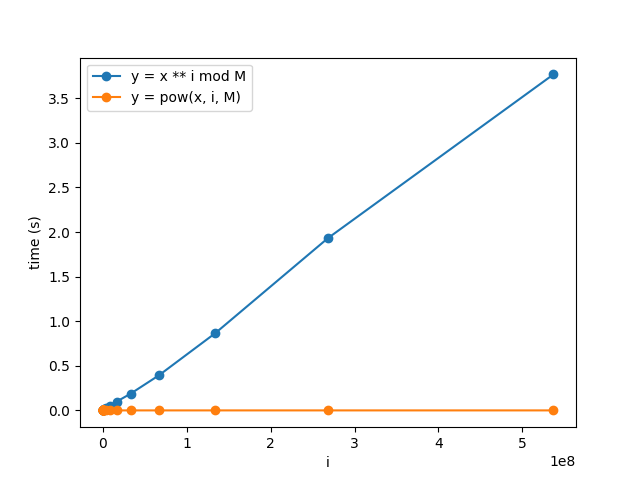
\includegraphics[]{pow_speed.png}
    \caption{Modular exponentiation speed comparison}
    \label{fig:pow_speed}
\end{figure}


\section{Discussion}

$10^{616}$ key space DH

Blum blum shub is slow and not practically secure (https://crypto.stackexchange.com/questions/3454/blum-blum-shub-vs-aes-ctr-or-other-csprngs)

\section{Conclusion}


% ========== References ========== %

\bibliographystyle{unsrtnat}
\bibliography{sources}

\end{document}



